

\section{datAcron Architecture}		
\frame
{		
	\frametitle{datAcron Architecture}
	\framesubtitle{}
	
	\begin{center}
		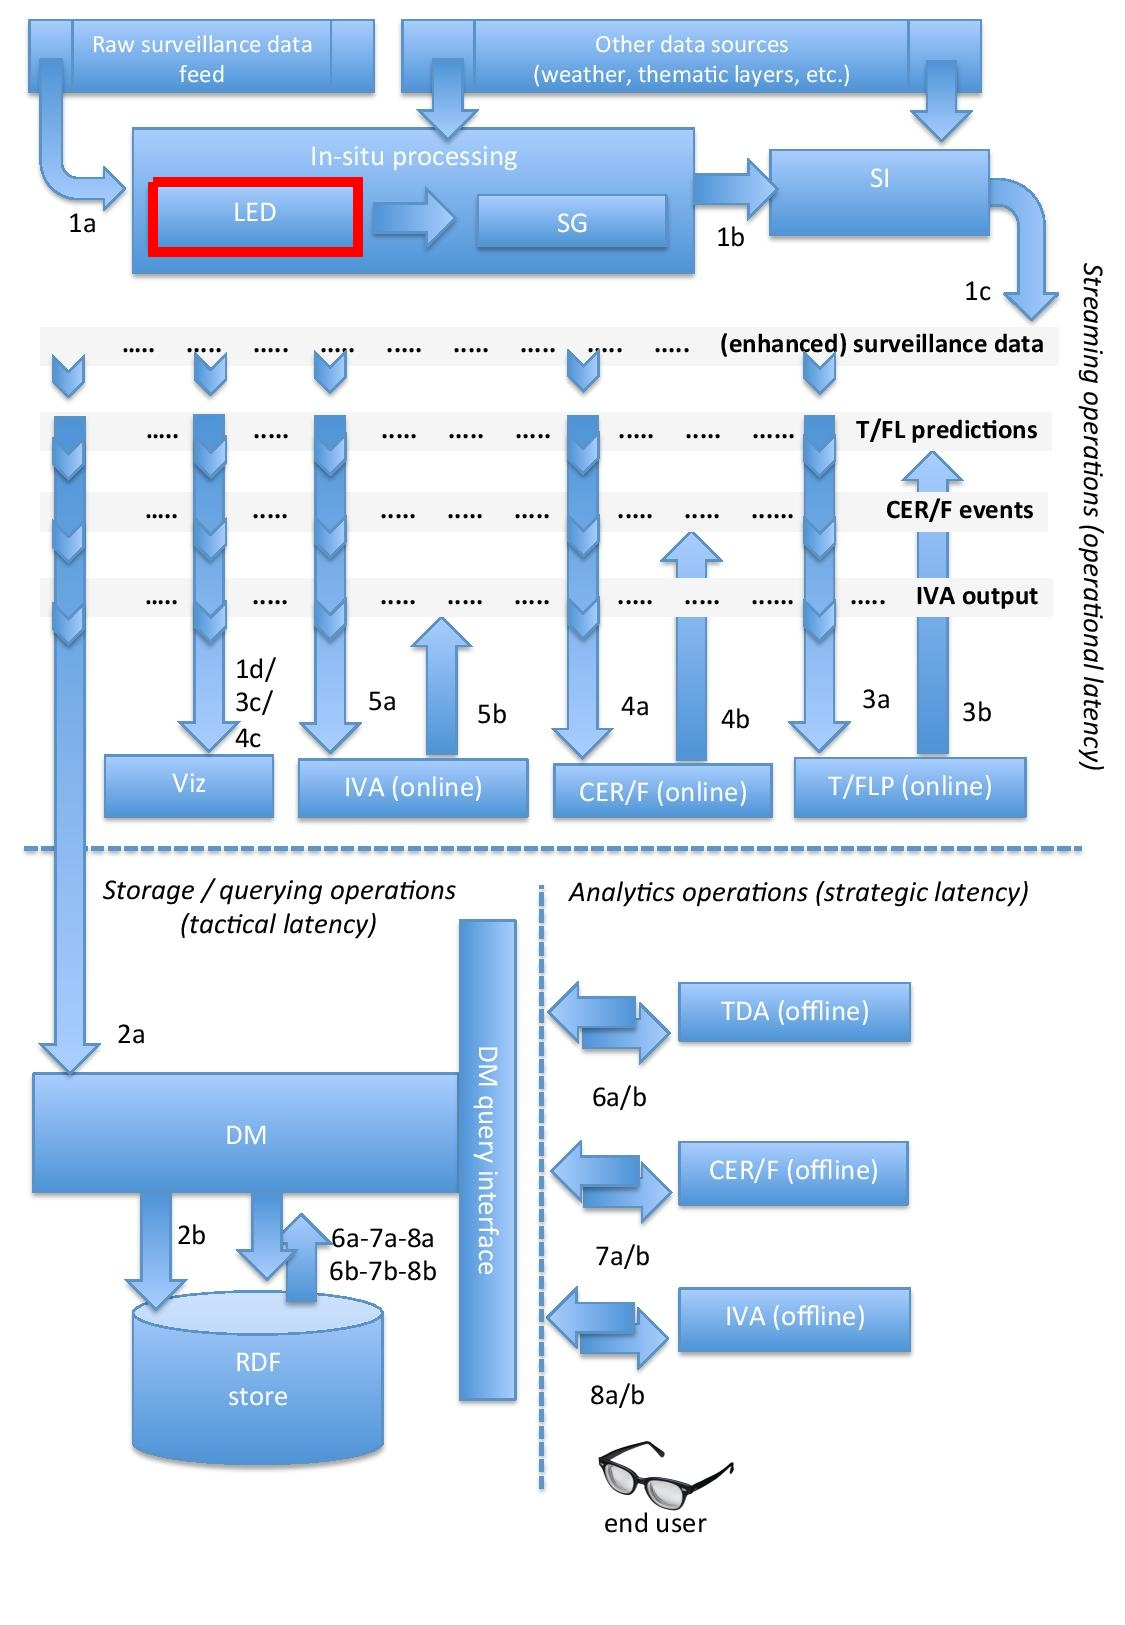
\includegraphics[width=.85\textwidth,height=.75\linewidth]{figures/arch1.jpg}\\
		.
	\end{center}
	
}

\section{Overview}
\frame
{
	\frametitle{In-situ (LED Component) \footnote{ github.com/ehabqadah/in-situ-processing-datAcron}}
	\framesubtitle{Overview}
		\begin{center}
			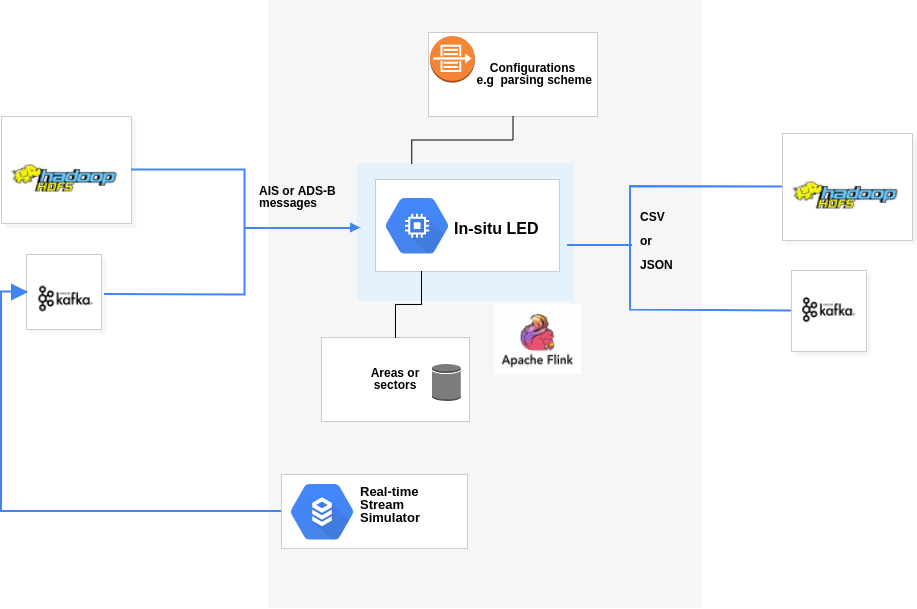
\includegraphics[scale=.32,left]{figures/insitu.png}\\
			.
		\end{center}
}


\frame
{
	\frametitle{In-situ LED}
	\framesubtitle{Functionalities}
	\begin{itemize}[]
	\item Trajectory enrichment: computing trajectory statistics  such as min/max/mean/var speed.
    \item Monitoring of AIS messages against areas information (detected areas)
	\item Derivation of low-level events for area entering and leaving

		
	\end{itemize}
}

\frame
{
	\frametitle{Real-time stream simulator}
	
	\begin{itemize}[]
		\item<1-> Read raw AIS File to  generate a reply stream
		
		\item<1 -> Reconstruct the trajectories and use the actual time difference between the points to replay origin stream
		
		\item<1 -> $delayScale$ parameter to scale up/down the out stream rate
		
	
	\end{itemize}
}


\section{Output Scheme}		
\frame
{		
\frametitle{Output CSV scheme (29 fields)}
\framesubtitle{}

\begin{center}
	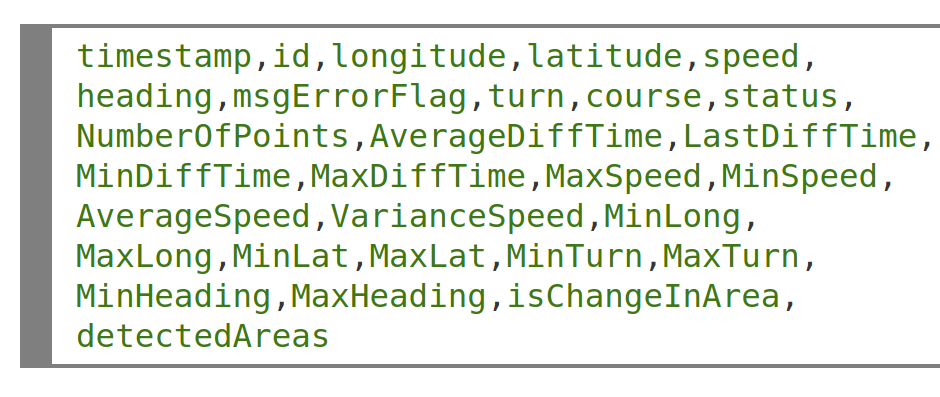
\includegraphics[scale=.32,left]{figures/insitu_output.png}\\
	.
\end{center}

}



\section{Deployment and Integration }

\begin{frame}
\frametitle{Deployment}
\begin{columns}
\begin{column}{0.5\textwidth}
  \begin{itemize}
  \item<1-> From deployment on a single VM machine 
  \end{itemize}
\end{column}
\begin{column}{0.5\textwidth}  
  \begin{itemize}
  \item<1-> To deployment on the YARN datAcron cluster ($10\ nodes\ X\ 8\ cores$)
  \end{itemize}
\end{column}
\end{columns}
\end{frame}





\frame
{	
	\frametitle{In-situ deployment on datAcron YARN cluster}

	\begin{center}
		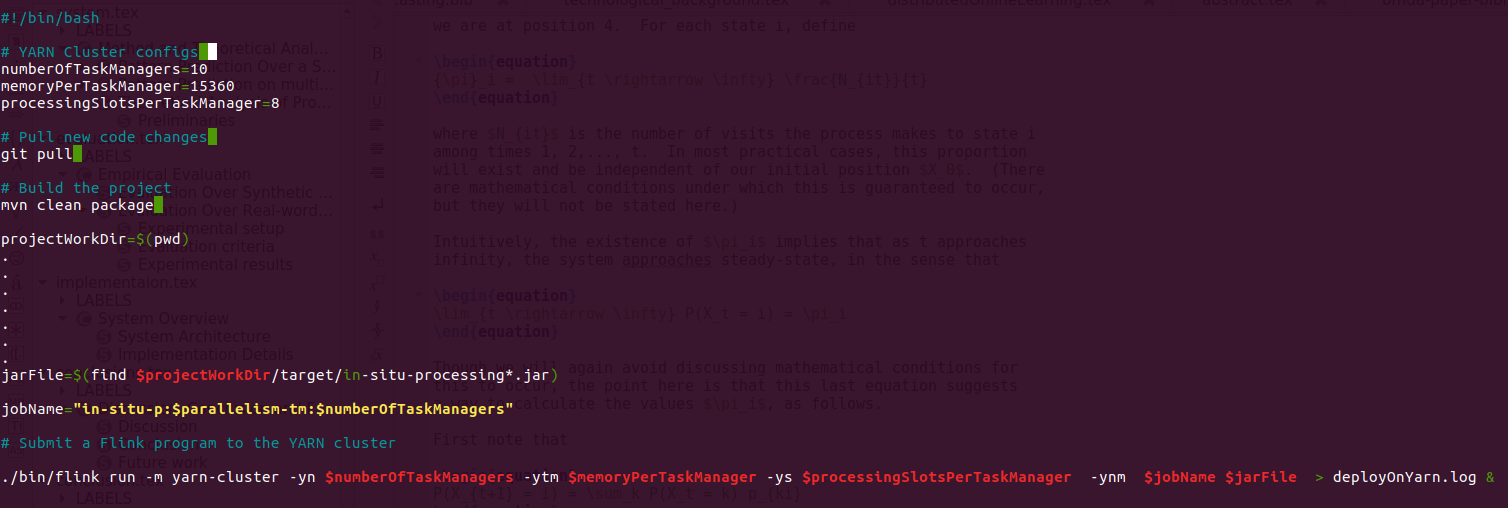
\includegraphics[width=.7\textwidth,height=.5\linewidth]{figures/deploy.png}
		.
	\end{center}
}


\section{Performance on YARN cluster}
\frame
{	
	\frametitle{In-situ Performance}
	\framesubtitle{Throughput on datAcron YARN cluster}
		\begin{center}
		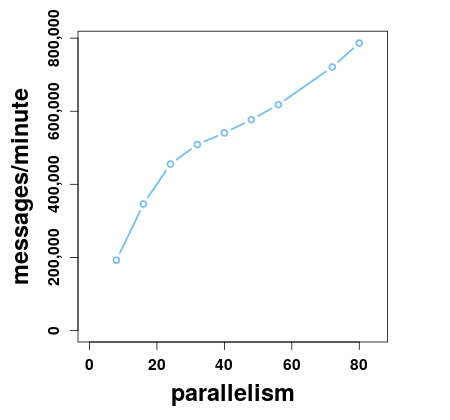
\includegraphics[width=.95\textwidth,height=.7\linewidth]{figures/throughput.png}
		.
	\end{center}
}


\section{Conclusion}
\frame
{	\frametitle{Conclusion}
	LED in-situ processing resources/CPU consumption and delay
	can be neglected
}